\documentclass[tikz,border=10pt]{standalone}
% Shared style for all Speed Demon diagrams: one palette, rounded white boxes,
% dark ink, white page (readable on GitHub light and dark).
\hyphenpenalty=10000 \exhyphenpenalty=10000 \tolerance=9999
\usepackage[T1]{fontenc}
\usepackage[scaled=0.95]{helvet}
\renewcommand{\familydefault}{\sfdefault}
\usepackage{tikz}
\usepackage{pgfplots}
\pgfplotsset{compat=1.16}
\usetikzlibrary{arrows.meta,positioning,shapes.geometric,fit,backgrounds,calc}

\definecolor{ink}{HTML}{1F2937}
\definecolor{mute}{HTML}{6B7280}
\definecolor{rule}{HTML}{9CA3AF}
\definecolor{cA}{HTML}{2563EB}   % Track A  blue
\definecolor{cB}{HTML}{D97706}   % Track B  amber
\definecolor{cC}{HTML}{059669}   % Track C  green
\definecolor{cD}{HTML}{7C3AED}   % Track D  violet
\definecolor{warn}{HTML}{DC2626} % fallback / redo path
\definecolor{wash}{HTML}{F3F4F6}

\tikzset{
  every node/.style={font=\small, text=ink},
  >={Stealth[length=2.4mm,width=1.8mm]},
  box/.style={draw=ink, fill=white, rounded corners=3pt, line width=0.7pt,
    align=center, inner sep=5pt, minimum height=12mm, text width=#1},
  box/.default=44mm,
  accent/.style={draw=#1, line width=1.2pt},
  accent/.default=cA,
  hl/.style={fill=#1!10, draw=#1, line width=1.1pt},
  dec/.style={diamond, aspect=2.6, draw=ink, fill=white, line width=0.7pt,
    align=center, inner sep=2pt, text width=#1},
  dec/.default=34mm,
  arr/.style={->, line width=0.9pt, color=ink},
  redo/.style={->, line width=0.9pt, color=warn, dash pattern=on 4pt off 3pt},
  lab/.style={font=\footnotesize, text=mute, inner sep=2pt},
  grp/.style={draw=#1, dashed, line width=0.9pt, rounded corners=6pt, inner sep=9pt,
    fill=#1!4},
  grp/.default=mute,
  grplabel/.style={font=\footnotesize\bfseries, text=#1, inner sep=2pt},
  show background rectangle,
  background rectangle/.style={fill=white, rounded corners=0pt},
}
\pgfplotsset{
  every axis/.append style={font=\small, tick label style={font=\footnotesize},
    axis line style={ink}, tick style={ink}, grid style={rule!50},
    label style={font=\small}, title style={font=\small\bfseries}},
}

% node text: \nt{title}{detail}
\newcommand{\nt}[2]{\textbf{#1}\par\vspace{1pt}{\footnotesize #2}}

\begin{document}
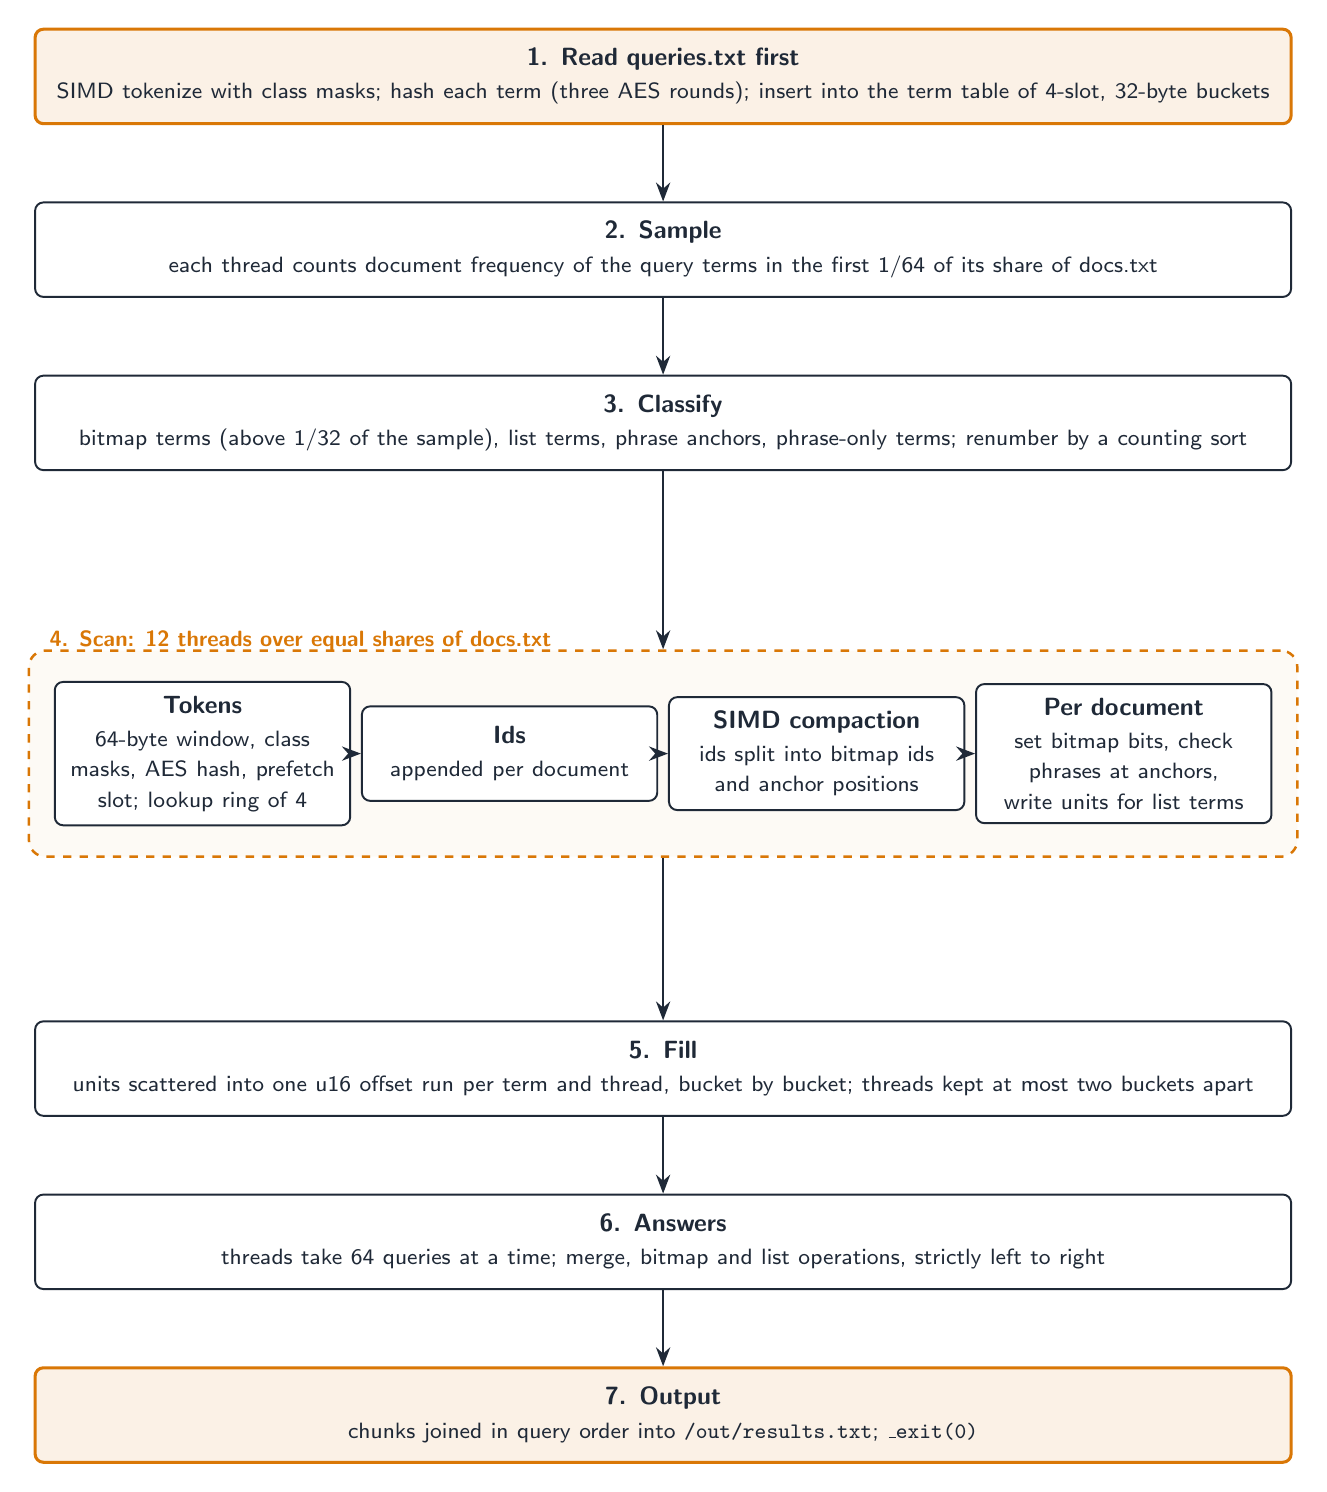
\begin{tikzpicture}
  \def\w{156mm}
  \node[box=\w, hl=cB] (q) at (0,0) {\nt{1. Read queries.txt first}{SIMD tokenize with class masks; hash each term (three AES rounds); insert into the term table of 4-slot, 32-byte buckets}};
  \node[box=\w] (s) at (0,-2.2) {\nt{2. Sample}{each thread counts document frequency of the query terms in the first 1/64 of its share of docs.txt}};
  \node[box=\w] (c) at (0,-4.4) {\nt{3. Classify}{bitmap terms (above 1/32 of the sample), list terms, phrase anchors, phrase-only terms; renumber by a counting sort}};

  % scan group
  \node[box=34mm] (t1) at (-5.85,-8.6) {\nt{Tokens}{64-byte window, class masks, AES hash, prefetch slot; lookup ring of 4}};
  \node[box=34mm] (t2) at (-1.95,-8.6) {\nt{Ids}{appended per document}};
  \node[box=34mm] (t3) at (1.95,-8.6) {\nt{SIMD compaction}{ids split into bitmap ids and anchor positions}};
  \node[box=34mm] (t4) at (5.85,-8.6) {\nt{Per document}{set bitmap bits, check phrases at anchors, write units for list terms}};
  \begin{scope}[on background layer]
    \node[grp=cB, fit=(t1)(t2)(t3)(t4), inner ysep=11pt] (scan) {};
  \end{scope}
  \node[grplabel=cB, anchor=south west] at ([xshift=2mm,yshift=-1mm]scan.north west) {4. Scan: 12 threads over equal shares of docs.txt};

  \node[box=\w] (f) at (0,-12.6) {\nt{5. Fill}{units scattered into one u16 offset run per term and thread, bucket by bucket; threads kept at most two buckets apart}};
  \node[box=\w] (a) at (0,-14.8) {\nt{6. Answers}{threads take 64 queries at a time; merge, bitmap and list operations, strictly left to right}};
  \node[box=\w, hl=cB] (o) at (0,-17.0) {\nt{7. Output}{chunks joined in query order into \texttt{/out/results.txt}; \texttt{\_exit(0)}}};

  \draw[arr] (q) -- (s);
  \draw[arr] (s) -- (c);
  \draw[arr] (c) -- (scan.north);
  \draw[arr] (t1) -- (t2);
  \draw[arr] (t2) -- (t3);
  \draw[arr] (t3) -- (t4);
  \draw[arr] (scan.south) -- (f);
  \draw[arr] (f) -- (a);
  \draw[arr] (a) -- (o);
\end{tikzpicture}
\end{document}
